\documentclass{article}

\usepackage{microtype}
\usepackage{graphicx}
\usepackage{adjustbox}
\usepackage{subcaption}
\usepackage{booktabs}
\usepackage{amsmath,amssymb,mathtools}
\usepackage{xcolor}
\usepackage{tikz}
\usepackage{hyperref}
\usepackage[accepted]{icml2026}
\setcitestyle{numbers,square,comma,sort&compress}

\usetikzlibrary{arrows.meta,positioning,calc,fit,shapes.geometric}

\definecolor{bluebg}{RGB}{240,247,251}
\definecolor{blueline}{RGB}{46,93,122}
\definecolor{maskbg}{RGB}{252,246,230}
\definecolor{maskline}{RGB}{166,112,32}
\definecolor{greenbg}{RGB}{237,248,241}
\definecolor{greenline}{RGB}{55,130,88}
\definecolor{controlbg}{RGB}{247,241,249}
\definecolor{controlline}{RGB}{124,79,137}
\definecolor{statebg}{RGB}{245,246,247}
\definecolor{stateline}{RGB}{94,101,108}

\newcommand{\diagramfont}{\scriptsize}

\tikzset{
  box/.style={draw=blueline, fill=bluebg, rounded corners=2pt,
    align=center, inner sep=4pt, font=\diagramfont},
  tinybox/.style={draw=blueline, fill=bluebg, rounded corners=2pt,
    align=center, inner sep=3pt, font=\diagramfont},
  maskbox/.style={draw=maskline, fill=maskbg, rounded corners=2pt,
    align=center, inner sep=3pt, font=\diagramfont},
  greenbox/.style={draw=greenline, fill=greenbg, rounded corners=2pt,
    align=center, inner sep=3pt, font=\diagramfont},
  dataflow/.style={draw=blueline, fill=bluebg, rounded corners=2pt,
    align=center, inner sep=3pt, text width=20mm, minimum height=8mm,
    font=\diagramfont},
  probflow/.style={draw=maskline, fill=maskbg, rounded corners=2pt,
    align=center, inner sep=3pt, text width=20mm, minimum height=8mm,
    font=\diagramfont},
  modelstage/.style={draw=greenline, fill=greenbg, rounded corners=2pt,
    align=center, inner sep=3pt, text width=20mm, minimum height=8mm,
    font=\diagramfont},
  controlstage/.style={draw=controlline, fill=controlbg, rounded corners=2pt,
    align=center, inner sep=3pt, text width=20mm, minimum height=8mm,
    font=\diagramfont},
  sysstage/.style={draw=stateline, fill=statebg, rounded corners=2pt,
    align=center, inner sep=3pt, text width=21mm, minimum height=7mm,
    font=\diagramfont},
  decision/.style={diamond, draw=controlline, fill=controlbg, aspect=1.55,
    align=center, inner sep=1pt, font=\diagramfont},
  flowlabel/.style={font=\diagramfont, fill=white, inner sep=1pt},
  arrow/.style={-{Latex[length=2mm]}, thick},
  reversearrow/.style={{Latex[length=2mm]}-, thick, dashed},
  feedback/.style={-{Latex[length=1.8mm]}, thick, dashed, draw=stateline}
}

\newcommand{\mask}{\ensuremath{\mathtt{[M]}}}
\newcommand{\Vocab}{\mathcal{V}}
\newcommand{\Data}{\mathcal{D}}
\newcommand{\Latency}{\operatorname{Latency}}
\newcommand{\NFE}{\operatorname{NFE}}

\icmltitlerunning{Diffusion Language Models: Foundations for Algorithm Design}

\begin{document}

\twocolumn[
\icmltitle{Diffusion Language Models: Foundations for Algorithm Design}

\begin{icmlauthorlist}
\icmlauthor{Working Group Notes}{wiki}
\end{icmlauthorlist}

\icmlaffiliation{wiki}{llmwiki research notes}
\icmlcorrespondingauthor{Working Group Notes}{llmwiki internal draft}

\icmlkeywords{Diffusion Language Models, Discrete Diffusion, Flow Matching,
Masked Diffusion, Inference, Optimization}

\vskip 0.3in
]

\printAffiliationsAndNotice{}

\begin{abstract}
Diffusion language modeling is not one algorithmic problem.  Continuous
diffusion, flow matching, general discrete diffusion, and absorbing-mask DLMs
change different mathematical objects.  This note keeps only the foundations
needed for team discussion: the process, learned target, executable sampler,
optimization surface, and falsification contract.
\end{abstract}

\section{First-Principles Object}

The phrase ``solve the diffusion process'' is ambiguous in language
modeling: it may mean numerical integration in continuous space, reverse
simulation of a discrete Markov process, path design and vector-field learning,
or control of a masked-DLM sampler.  Before discussing algorithms, name four
objects:
\[
\text{state},\quad \text{learned conditional},\quad
\text{action},\quad \text{budget}.
\]

\begin{figure}[t]
\centering
\begin{adjustbox}{max width=\columnwidth,center}
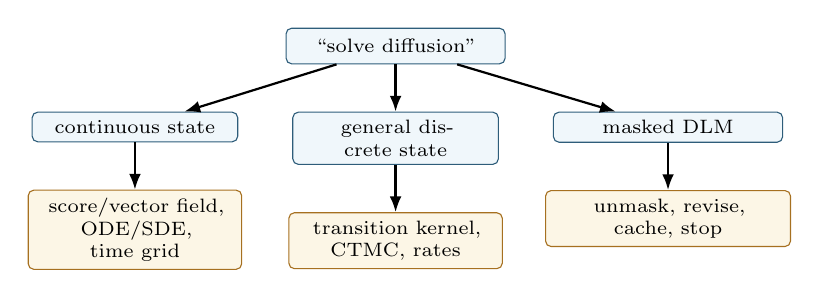
\begin{tikzpicture}[node distance=6mm and 6mm]
  \node[box, text width=25mm] (q) {``solve diffusion''};
  \node[tinybox, text width=24mm, below left=of q] (cont)
    {continuous state};
  \node[tinybox, text width=24mm, below=of q] (disc)
    {general discrete state};
  \node[tinybox, text width=27mm, below right=of q] (mask)
    {masked DLM};
  \node[maskbox, text width=25mm, below=of cont] (conta)
    {score/vector field, ODE/SDE, time grid};
  \node[maskbox, text width=25mm, below=of disc] (disca)
    {transition kernel, CTMC, rates};
  \node[maskbox, text width=29mm, below=of mask] (maska)
    {unmask, revise, cache, stop};
  \draw[arrow] (q) -- (cont);
  \draw[arrow] (q) -- (disc);
  \draw[arrow] (q) -- (mask);
  \draw[arrow] (cont) -- (conta);
  \draw[arrow] (disc) -- (disca);
  \draw[arrow] (mask) -- (maska);
\end{tikzpicture}
\end{adjustbox}
\caption{Three distinct meanings of solving diffusion.}
\label{fig:interfaces}
\end{figure}

\section{Transport Foundations}

\subsection{Continuous reference point}

For continuous data, a common variance-preserving marginal is
\begin{equation}
z_t=\sqrt{\alpha_t}x+\sqrt{1-\alpha_t}\epsilon,
\qquad \epsilon\sim\mathcal{N}(0,I),
\label{eq:continuous}
\end{equation}
where the schedule moves clean data toward a tractable prior.  A learned score
induces a reverse SDE or probability-flow ODE; inference chooses its solver
and time grid \citep{ho2020ddpm,lu2022dpmsolver}.  Continuous text diffusion
applies this geometry to embeddings or latent vectors \citep{li2022diffusionlm}.

\subsection{Flow matching}

Flow matching (FM) learns the velocity of a chosen probability path rather
than a score.  If a conditional path has velocity $u_t(x_t\mid x_1)$, the
simulation-free objective is
\begin{equation}
\mathcal{L}_{\mathrm{FM}}
=\mathbb{E}_{t,x_1,x_t}
\left\|v_\theta(x_t,t)-u_t(x_t\mid x_1)\right\|_2^2.
\label{eq:flow-matching}
\end{equation}
Sampling integrates \(\dot z_t=v_\theta(z_t,t)\).  Diffusion paths are a
special case, whereas optimal-transport paths need not be diffusions
\citep{lipman2023flow}.

Discrete Flow Matching (DFM) instead defines probability paths and velocities
over categorical states, making the coupling, scheduler, and CTMC sampler
explicit \citep{gat2024dfm,shaul2024generalpaths}.  Dirichlet and Fisher flow
matching provide alternative simplex or statistical-manifold geometries for
discrete sequences \citep{stark2024dirichlet,davis2024fisher}.  Thus flow
matching changes the path and training target; it does not eliminate the
inference-time discretization problem.

\subsection{Discrete Markov diffusion}

Let a token be a one-hot vector in a vocabulary \(\Vocab\).  D3PM defines a
forward Markov chain using categorical transition matrices \(Q_t\):
\begin{align}
q(z_t\mid z_{t-1}) &= \operatorname{Cat}(z_t;Q_tz_{t-1}),\\
q(z_t\mid x) &= \operatorname{Cat}(z_t;\bar Q_tx),
\quad \bar Q_t=Q_tQ_{t-1}\cdots Q_1.
\label{eq:d3pm}
\end{align}
The known forward process gives \(q(z_{t-1}\mid z_t,x)\).  A neural model
replaces the unknown clean \(x\) at generation time.  Its NELBO contains
\begin{equation}
\mathcal{L}_{\mathrm{diff}}
=\sum_t\mathbb{E}_{q(z_t\mid x)}
 D_{\mathrm{KL}}\!\left[q(z_{t-1}\mid z_t,x)
 \Vert p_\theta(z_{t-1}\mid z_t)\right].
\label{eq:discrete-elbo}
\end{equation}
D3PM permits uniform, structured, or absorbing transitions
\citep{austin2021d3pm}.  Continuous-time variants use a CTMC rate matrix;
SEDD estimates ratios needed by the reverse process
\citep{campbell2022continuous,lou2024sedd}.

\section{Absorbing-Mask Language Diffusion}

\subsection{Forward process}

Introduce a special absorbing mask state \(m=\mask\).  For a clean token
\(x\), masked diffusion uses
\begin{equation}
q(z_t\mid x)=\operatorname{Cat}
\left(z_t;\alpha_t x+(1-\alpha_t)m\right),
\label{eq:mask-forward}
\end{equation}
with \(\alpha_0\approx1\), \(\alpha_1\approx0\), and
\(\alpha_t\) decreasing.  A token either remains clean or jumps to the mask;
after it is masked in the forward process, it stays masked.  The process is
applied independently to response positions, while conditioning or prompt
tokens remain visible.

For \(0\le s<t\le1\), define the categorical parameter
\begin{equation}
r_{s,t}(x)=
\frac{(1-\alpha_s)m+(\alpha_s-\alpha_t)x}{1-\alpha_t}.
\label{eq:mask-mixture}
\end{equation}
The posterior has a simple interpretation.  If \(z_t\neq m\), then the
earlier state must equal \(z_t\).  If \(z_t=m\), the earlier state is either
still masked or equal to the clean token:
\begin{equation}
q(z_s\mid z_t,x)=
\begin{cases}
\delta_{z_t}, & z_t\neq m,\\[2pt]
\operatorname{Cat}(z_s;r_{s,t}(x)), & z_t=m.
\end{cases}
\label{eq:mask-posterior}
\end{equation}

Figure~\ref{fig:dlm-process} separates one-shot training corruption from the
iterative generation loop.

\begin{figure*}[t]
\centering
\resizebox{\textwidth}{!}{%
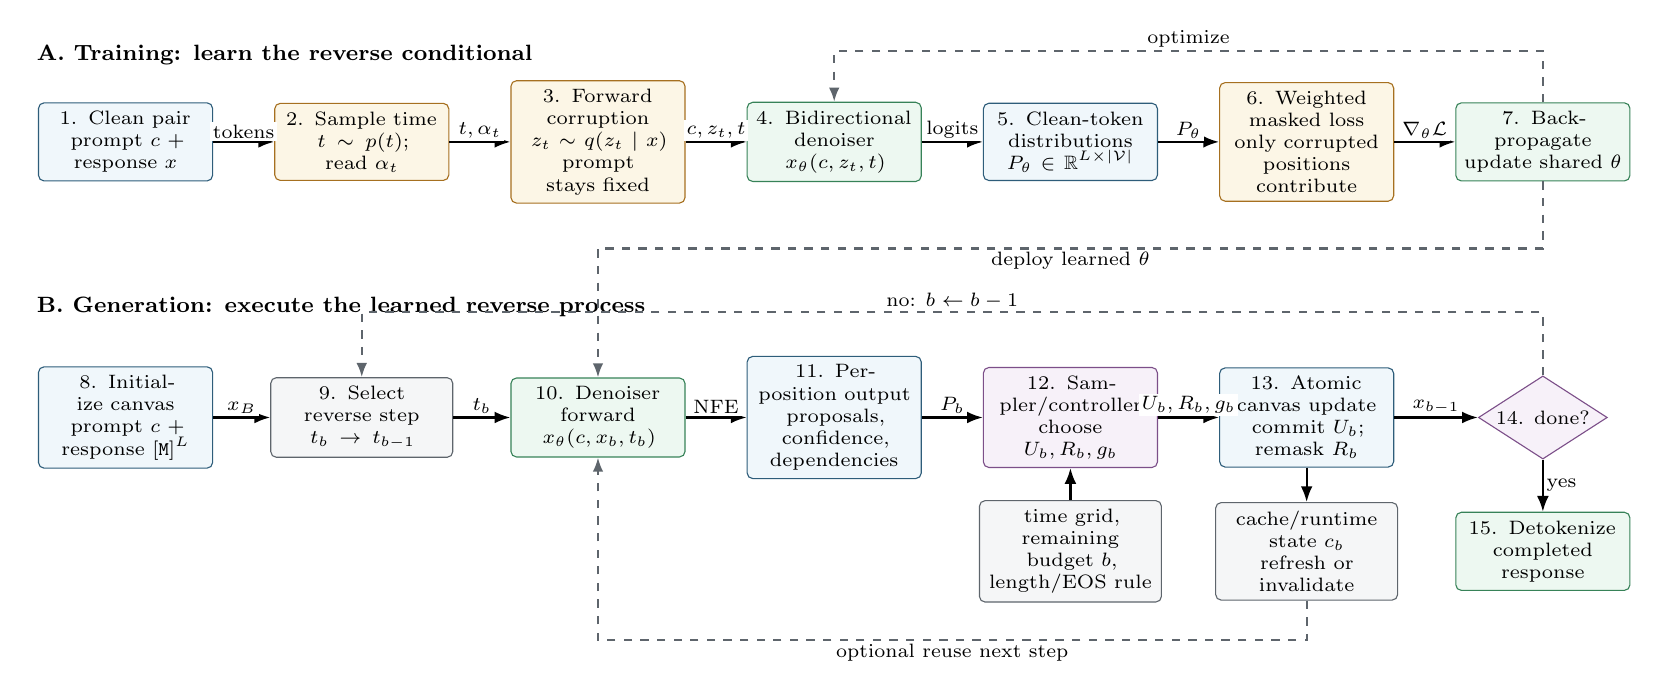
\begin{tikzpicture}[x=1cm,y=1cm]
  \node[font=\footnotesize\bfseries, anchor=west] at (-1.25,5.45)
    {A. Training: learn the reverse conditional};
  \node[dataflow] (clean) at (0,4.35)
    {1. Clean pair\\prompt $c$ + response $x$};
  \node[probflow] (time) at (3.0,4.35)
    {2. Sample time\\$t\sim p(t)$; read $\alpha_t$};
  \node[probflow] (corrupt) at (6.0,4.35)
    {3. Forward corruption\\$z_t\sim q(z_t\mid x)$\\prompt stays fixed};
  \node[modelstage] (trainmodel) at (9.0,4.35)
    {4. Bidirectional denoiser\\$x_\theta(c,z_t,t)$};
  \node[dataflow] (trainprob) at (12.0,4.35)
    {5. Clean-token distributions\\$P_\theta\in\mathbb{R}^{L\times|\Vocab|}$};
  \node[probflow] (loss) at (15.0,4.35)
    {6. Weighted masked loss\\only corrupted positions contribute};
  \node[modelstage] (update) at (18.0,4.35)
    {7. Backpropagate\\update shared $\theta$};

  \draw[arrow] (clean) -- node[flowlabel,above]{tokens} (time);
  \draw[arrow] (time) -- node[flowlabel,above]{$t,\alpha_t$} (corrupt);
  \draw[arrow] (corrupt) -- node[flowlabel,above]{$c,z_t,t$} (trainmodel);
  \draw[arrow] (trainmodel) -- node[flowlabel,above]{logits} (trainprob);
  \draw[arrow] (trainprob) -- node[flowlabel,above]{$P_\theta$} (loss);
  \draw[arrow] (loss) -- node[flowlabel,above]{$\nabla_\theta\mathcal{L}$} (update);
  \draw[feedback] (update.north) -- ++(0,0.65) -|
    node[flowlabel,near start,above]{optimize} (trainmodel.north);

  \node[font=\footnotesize\bfseries, anchor=west] at (-1.25,2.25)
    {B. Generation: execute the learned reverse process};
  \node[dataflow] (init) at (0,0.85)
    {8. Initialize canvas\\prompt $c$ + response $\mask^L$};
  \node[sysstage] (step) at (3.0,0.85)
    {9. Select reverse step\\$t_b\rightarrow t_{b-1}$};
  \node[modelstage] (infermodel) at (6.0,0.85)
    {10. Denoiser forward\\$x_\theta(c,x_b,t_b)$};
  \node[dataflow] (scores) at (9.0,0.85)
    {11. Per-position output\\proposals, confidence, dependencies};
  \node[controlstage] (policy) at (12.0,0.85)
    {12. Sampler/controller\\choose $U_b,R_b,g_b$};
  \node[dataflow] (canvas) at (15.0,0.85)
    {13. Atomic canvas update\\commit $U_b$; remask $R_b$};
  \node[decision] (done) at (18.0,0.85) {14. done?};

  \node[sysstage] (budget) at (12.0,-0.85)
    {time grid, remaining budget $b$, length/EOS rule};
  \node[sysstage] (cache) at (15.0,-0.85)
    {cache/runtime state $c_b$\\refresh or invalidate};
  \node[greenbox, text width=20mm] (output) at (18.0,-0.85)
    {15. Detokenize\\completed response};

  \draw[arrow] (init) -- node[flowlabel,above]{$x_B$} (step);
  \draw[arrow] (step) -- node[flowlabel,above]{$t_b$} (infermodel);
  \draw[arrow] (infermodel) -- node[flowlabel,above]{NFE} (scores);
  \draw[arrow] (scores) -- node[flowlabel,above]{$P_b$} (policy);
  \draw[arrow] (policy) -- node[flowlabel,above]{$U_b,R_b,g_b$} (canvas);
  \draw[arrow] (canvas) -- node[flowlabel,above]{$x_{b-1}$} (done);
  \draw[arrow] (done) -- node[flowlabel,right]{yes} (output);
  \draw[feedback] (done.north) -- ++(0,0.80) -|
    node[flowlabel,near start,above]{no: $b\leftarrow b-1$} (step.north);
  \draw[feedback] (update.south) -- ++(0,-0.85) -|
    node[flowlabel,near start,below]{deploy learned $\theta$} (infermodel.north);
  \draw[arrow] (budget) -- (policy);
  \draw[arrow] (canvas) -- (cache);
  \draw[feedback] (cache.south) -- ++(0,-0.50) -|
    node[flowlabel,near start,below]{optional reuse next step} (infermodel.south);
\end{tikzpicture}
}
\caption{Masked-DLM lifecycle.  Training corrupts once; generation iterates
denoising and canvas updates.  Colors distinguish data (blue), known
operations (orange), model/output (green), control (violet), and state (gray).}
\label{fig:dlm-process}
\end{figure*}

\subsection{Reverse parameterization and training}

Because clean \(x\) is unknown during generation, a denoiser
\(x_\theta(z_t,t)\) predicts a distribution over clean tokens.  Substituting
this prediction into Equation~\ref{eq:mask-posterior} defines
\(p_\theta(z_s\mid z_t)\).  MDLM additionally enforces zero probability for
the mask as a clean token and carries already unmasked tokens forward.  These
choices simplify the continuous-time NELBO to
\begin{equation}
\mathcal{L}_{\mathrm{MDLM}}
=\mathbb{E}_{x,t,z_t}
\left[\frac{\alpha'_t}{1-\alpha_t}
\log \langle x_\theta(z_t,t),x\rangle\right].
\label{eq:mdlm-loss}
\end{equation}
Since \(\alpha'_t<0\), minimizing this expression is a weighted masked-token
cross-entropy objective.  This connection explains why BERT-like bidirectional
Transformers can parameterize generative masked diffusion, but it does not
make an ordinary masked language model a DLM automatically
\citep{he2023diffusionbert,zheng2024rdm,sahoo2024mdlm}.

\section{Sampler as the Optimization Object}

The denoiser returns conditional token distributions; the sampler turns them
into state changes.  The lifecycle in Figure~\ref{fig:dlm-process} is therefore
the operational algorithm: observe the current canvas, run the denoiser, choose
which tokens to commit or revise, update state, and stop under a budget.

For a masked DLM, a compact post-forward observation is
\begin{equation}
s_b=(x_b,M_b,P_b,h_b,c_b,b),
\label{eq:state}
\end{equation}
where \(M_b\) is the mask set, \(P_b\) the current model output, \(h_b\)
trajectory history, \(c_b\) cache/system state, and \(b\) remaining budget.
An action can be represented as
\begin{equation}
a_b=(U_b,R_b,g_b,\mathrm{stop}),
\label{eq:action}
\end{equation}
where \(U_b\) commits positions, \(R_b\) revises or verifies positions, and
\(g_b\) selects a compute mode.  This is a history-augmented control problem,
not automatically a small MDP: token actions are combinatorial and final
quality is observed late.  The minimal matched-budget comparison is
\begin{equation}
\max_\pi\ \mathbb{E}_{q\sim\Data}[Q_\pi(q)]
\quad\text{s.t.}\quad \sum_b\NFE_b\le B.
\label{eq:budget}
\end{equation}
Wall-clock claims additionally require synchronized p50/p95 latency, memory,
batching, and policy overhead \citep{gwak2026acceleration}.

\begin{table}[H]
\caption{Where an algorithm can act.}
\label{tab:surfaces}
\centering
\footnotesize
\begin{tabular}{p{15mm}p{24mm}p{27mm}}
\toprule
Layer & Decision variable & Falsifying question \\
\midrule
Path & transition/rate, mask schedule & Is the gain just a different training target? \\
Model & backbone, time conditioning & Does it hold at matched parameters/training? \\
Sampler & time grid, update set, revision & Does it beat matched NFE and wall-clock cost? \\
Length & canvas, EOS, block factorization & Are failures hidden as unfinished masks? \\
System & cache, batching, kernels & Are states still valid after revisions? \\
\bottomrule
\end{tabular}
\end{table}

Three pitfalls usually decide whether an idea is real.  A fixed canvas needs a
length mechanism \citep{sahoo2024mdlm,arriola2025block,cheng2026length};
independent token marginals do not guarantee jointly safe parallel commits; and
remasking changes both the transition rule and cache validity.

\section{Historical and Model Map}

Iterative masked decoding predates modern DLMs; continuous diffusion, discrete
diffusion, and flow matching developed as related but distinct paths.
Figure~\ref{fig:timeline} is a cited reading map, not a lineage claim
\citep{yu2025survey}.

\begin{figure}[t]
\centering
\begin{adjustbox}{max width=\columnwidth,center}
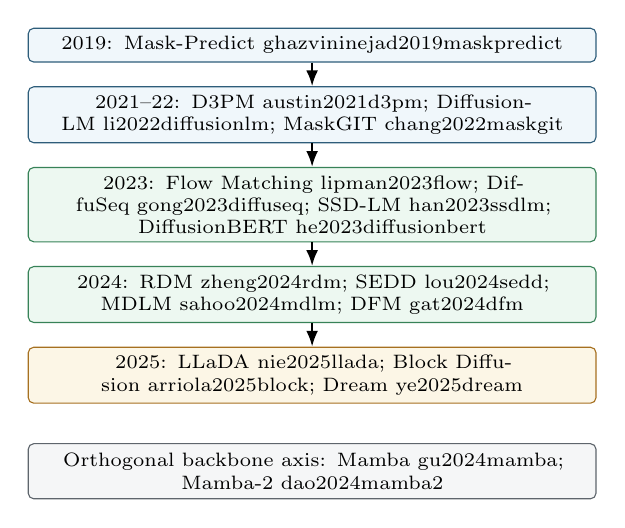
\begin{tikzpicture}[node distance=3mm]
  \node[tinybox, text width=70mm] (a)
    {2019: Mask-Predict~\citep{ghazvininejad2019maskpredict}};
  \node[tinybox, text width=70mm, below=of a] (b)
    {2021--22: D3PM~\citep{austin2021d3pm};
    Diffusion-LM~\citep{li2022diffusionlm};
    MaskGIT~\citep{chang2022maskgit}};
  \node[greenbox, text width=70mm, below=of b] (c)
    {2023: Flow Matching~\citep{lipman2023flow};
    DiffuSeq~\citep{gong2023diffuseq}; SSD-LM~\citep{han2023ssdlm};
    DiffusionBERT~\citep{he2023diffusionbert}};
  \node[greenbox, text width=70mm, below=of c] (d)
    {2024: RDM~\citep{zheng2024rdm}; SEDD~\citep{lou2024sedd};
    MDLM~\citep{sahoo2024mdlm}; DFM~\citep{gat2024dfm}};
  \node[maskbox, text width=70mm, below=of d] (e)
    {2025: LLaDA~\citep{nie2025llada};
    Block Diffusion~\citep{arriola2025block}; Dream~\citep{ye2025dream}};
  \node[sysstage, text width=70mm, below=5mm of e] (backbone)
    {Orthogonal backbone axis: Mamba~\citep{gu2024mamba};
    Mamba-2~\citep{dao2024mamba2}};
  \draw[arrow] (a) -- (b);
  \draw[arrow] (b) -- (c);
  \draw[arrow] (c) -- (d);
  \draw[arrow] (d) -- (e);
\end{tikzpicture}
\end{adjustbox}
\caption{A compact reading history.  Each named work has a numeric citation;
arrows order process-level foundations, while the gray box is a separate
backbone axis.}
\label{fig:timeline}
\end{figure}

Model families differ by probability path, representation, backbone,
factorization, length handling, and inference policy.  Mamba and Mamba-2 are
backbone choices rather than diffusion solvers \citep{gu2024mamba,dao2024mamba2}.
The large-model branch is currently represented by LLaDA, Block Diffusion, and
Dream \citep{nie2025llada,arriola2025block,ye2025dream}; newer work studies
trajectory mismatch, masked pretraining, and scaling
\citep{he2025mdpo,nie2026illada,sahoo2026scaling}.

\section{Research Constraints and Evidence}

Four constraints should stay visible during brainstorming.  First, metric
choice changes apparent speedup: few steps can look strong under perplexity
while sequence error grows with length \citep{feng2025theory}.  Second, masking
has process structure tied to known jump timing \citep{amin2025scud}.  Third, a
CTMC solver is not a token scheduler: solvers improve simulation, whereas
policies choose token actions \citep{ren2025fastsolvers}.  Finally, training and
inference paths can mismatch; random masks may not match generation canvases
\citep{he2025mdpo}.

An experiment must report the quality--cost frontier, not a single operating
point.  The minimum evidence is compact:

\begin{table}[H]
\caption{Minimum evidence for a DLM comparison.}
\label{tab:evaluation}
\centering
\footnotesize
\begin{tabular}{p{19mm}p{51mm}}
\toprule
Dimension & Report \\
\midrule
Model & checkpoint, training changes, tokenizer, time conditioning \\
Work & reverse steps, total model evaluations, extra scorers/branches \\
Latency & synchronized end-to-end p50/p95 and policy overhead \\
Memory & peak allocation and cache footprint \\
Length & prompt, canvas, generated length, EOS/completion rule \\
Quality & task metric, likelihood metric if relevant, completion rate \\
Robustness & second task, length regime, and preferably second model family \\
Controls & matched-cost baseline and signal-destroying ablation \\
\bottomrule
\end{tabular}
\end{table}

Common failure modes are unfinished masks, length ambiguity, confidence drift
across mask ratios, correlated token errors, stale caches, and gains that vanish
under matched compute.

\section{Research Gate}

\begin{center}
\fbox{\begin{minipage}{0.92\columnwidth}
\small
We change \emph{[layer/action]} using \emph{[signal]} under
\emph{[budget]}, because the matched baseline fails on
\emph{[diagnostic]}.  The idea is falsified if \emph{[matched-cost result]}.
If these fields cannot be filled, keep measuring or reading.
\end{minipage}}
\end{center}

\small
\bibliography{references}
\bibliographystyle{icml2026}

\end{document}
